{\color{secblue}\subsection{Implementation plan}}
{\color{secblue}\subsubsection{Overview}}
Being the TrackMe environment divided in components and subcomponents, the implementation plan will be performed by ordering and completing one or more subcomponent at a time, based on the dependencies between themselves. First the major tasks will be identified, then a more precise implementation plan will be presented.
{\color{secblue}\subsubsection{Major tasks}}
The most complex component is the server application, thus should be one of the most important concern. Considering the component view (sec 2.2), one can see that the general flow of interface usage is from left to right, with some parallel subcomponent in terms of interface usage. Considering this, the implementation of the server application is divided in 4 groups of subcomponents:

\begin{enumerate} 
\item the ones which communicate directly with the DB
\item the ones which use interfaces of the first group or that have no other dependencies
\item the ones which use interfaces of the second group
\item the dispatchers of incoming packets and the entry point
\end{enumerate}

Another major tasks which emerges is the protocol of the format of the packets. Such protocol should be completed as soon as possible, because by defining early the protocol, the various TrackMe applications can be developed in parallel with the server. This is possible because these applications don't contain almost any logic (and because of this, these components are not further analyzed in this section), and as prerequisite to develop them they need only to know how to send and receive information from the TrackMe server.

{\color{secblue}\subsubsection{Implementation Schedule}}
The components and subcomponents of the system are grouped and ordered in the following way:

\begin{enumerate}
\item ProviderAdapter and protocol of packets
\item D4HQueryService, D4HSingleUserRequestService, AutomatedSOSForwarder, T4RMapManager, T4RRunCreator, T4RJoinRunService
\item D4HSubscriptionProvider, D4HUpdateService, AuthenticationManager
\item D4HDispatcher, T4RDispatcher
\item GenericDispatcher, EntryPoint
\end{enumerate}

\paragraph{} Concerning the client applications, they can be developed indipendently after group 1 has been completed, in particular after the packet protocol has been defined. They do not require any particular order of developing, being indipendent each one from the other, and can be developed in parallel or sequentially depending on the available resources. 
\newline The protocol can be of any type or structure, such as a JSON, but should be kept in mind that given a possible growing amount of users, it should be defined paying attention to be as efficient as possible for a packet both on space usage, for a faster and lighter internet connection and time employed to extract information from it.


{\color{secblue}\subsection{Integration and test plan}}

{\color{secblue}\subsubsection{Overview}}
\paragraph{} The integration and test plans will be actuated in parallel with the implementation plan. In particular, a bottom-up approach will be adopted. Such approach has been chosen given the relative simplicity of the project.
Given the fact that in the TrackMe server environment each subcomponent in general relies on the service(s) provided by the implementation of the interface(s) required, and that each subcomponent has one functionality (or, if there are more than one, they are strictly related), the integration between each two subcomponents will be done only after the full completition of the one offering the interface.
\paragraph{} It is assumed that the AWS will be already available from the beginning of development, also because its adapter is the first subcomponent to be implemented on the server application. The same goes for the hospital calling service, which will be used to implement the AutomatedSOSForwarder.

{\color{secblue}\subsubsection{Integration plan}}
\paragraph{} The integration plan will proceed by grouping the subcomponents of the server application into several categories, accordingly to what has been described in the implementation plan. The categories are hence the following:
\newline
\begin{enumerate}
\item Database adapter
\item Components interfacing only the DB adapter
\item Components interfacing components of the second category
\item Service dispatchers
\item High level dispatcher
\item EntryPoint
\item TrackMe client applications
\end{enumerate}

The integration is further described, specifying which components have to be integrated to which other(s):
\paragraph {Database adapter} is composed only by the ProviderAdapter component, and must be integrated only with the AWS external component. The specific integration is:
\begin{itemize}
\item ProviderAdapter, AWS
\end{itemize}

\paragraph{Components interfacing only the DB adapter:} this group is constituted by all the subcomponents which directly use uniquely the ProviderAdapter (which is the DB adapter), and must be integrated with it. The full list of these subcomponents and their integration is:
\begin{itemize}
\item AuthenticationManager, ProviderAdapter
\item D4HQueryService, ProviderAdapter
\item D4HSingleUserRequestService, ProviderAdapter
\item T4RRunCreator, ProviderAdapter
\item T4RJoinRunService, ProviderAdapter
\end{itemize}

\paragraph{Components interfacing components of the second category:} here are included all subcomponents which have one or more dependencies with subcomponents of the previous group(s). Therefore they need to be integrated after the completition of the previously mentioned group. The full integration list is:
\begin{itemize}
\item D4HSubscriptionProvider, ProviderAdapter
\item D4HSubscriptionProvider, D4HQueryService
\item D4HUpdateService, ProviderAdapter
\item D4HUpdateService, AutomatedSOSForwarder
\item D4HUpdateService, T4RMapManager
\end{itemize}

\paragraph{Service dispatchers} are the dispatchers of the specific service: Data4Help and Track4Run (being AutomatedSOS exploiting Data4Help services). They need to be integrated with each subcomponent of their service, as they must channel the packet to the correct subcomponent. The full integration list is:
\begin{itemize}
\item D4HDispatcher, D4HSubscriptionProvider
\item D4HDispatcher, D4HQueryService
\item D4HDispatcher, D4HSingleUserRequestService
\item D4HDispatcher, D4HUpdateService
\item T4RDispatcher, T4RMapManager
\item T4RDispatcher, T4RRunCreator
\item T4RDispatcher, T4RJoinRunService
\end{itemize}

\paragraph{High level dispatcher} is only composed by the subcomponent GenericDispatcher, which must be integrated with the AuthenticationManager for indentification purposes and the previously mentioned service dispatchers, to which has to send packets according to the service. The full integration list is:
\begin{itemize}
\item GenericDispatcher, Authentication Manager
\item GenericDispatcher, D4HDispatcher
\item GenericDispatcher, T4RDispatcher
\end{itemize}

\paragraph{EntryPoint} is the last subcomponent to be integrated, and must only be integrated with the high level dispatcher. The precise integration is:
\begin{itemize}
\item EntryPoint, GenericDispatcher
\end{itemize}

\paragraph{TrackMe client applications:} finally, being the server application completely integrated at this point, each application can be integrated with the server one indipendently. In terms of high level components, the integration list is:
\begin{itemize}
\item Data4Help app, server application
\item Data4Help TP Edition application, server application
\item AutomatedSOS app, server application
\item Track4Run app, server application
\end{itemize}

{\color{secblue}\subsubsection{Integration details}}
In this section the previously mentioned groups of integration are furhter analyzed and graphically represented.
\newline Each dashed arrow represent the dependency and the verse of the integration. If multiple arrows point out from a component, that component will be integrated with two or more components separately. If multiple arrows point to a component, that component will be used in integration by multiple components in the same group.
In each group the order of integration is not relevant.\newline

\paragraph{Database adapter:} this group is composed by the ProviderAdapter component alone, and has the top priority in development because the subsequent subcomponents will require to interface themselves to the AWS database.
\begin{figure}[H]
    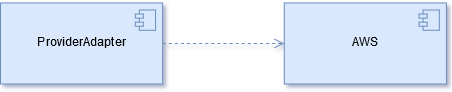
\includegraphics[width=.7\linewidth, keepaspectratio]{./Images/Section5/integration_g1.png}
    \centering
    \caption{Integration group 1}
    \label{fig:intg1}
 \end{figure}

\paragraph{Components interfacing only the DB adapter:} all the subcomponent in this group need to interface themselves directly to the DB (which has been abstracted through the ProviderAdapter), and do not require any other interface, thus are next in the dependencies hierarchy. All of them interfaces themselves to the same subcomponent, the ProviderAdapter:
\begin{figure}[H]
    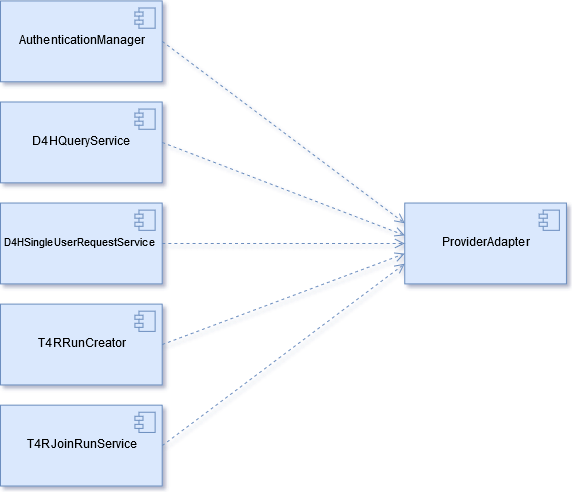
\includegraphics[width=.7\linewidth, keepaspectratio]{./Images/Section5/integration_g2.png}
    \centering
    \caption{Integration group 2}
    \label{fig:intg2}
 \end{figure}

\newpage
\paragraph{Components interfacing components of the second category:} these are the component next in the hierarchy, which use components of group 1 and/or 2.  These are services interfacing both the ProviderAdapter and which rely also on one or more subcomponents already developed.
\begin{figure}[H]
    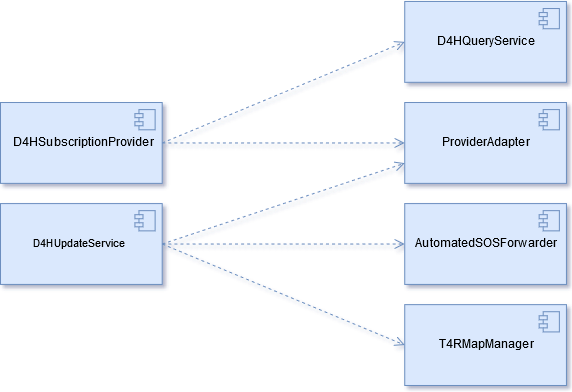
\includegraphics[width=.7\linewidth, keepaspectratio]{./Images/Section5/integration_g3.png}
    \centering
    \caption{Integration group 3}
    \label{fig:intg3}
 \end{figure}

\newpage
\paragraph[H]{Service dispatchers:} the service dispatchers are the two lower-level dispatcher designated to forward packets of a service to the specific task of a service. Therefore they must rely on such tasks, implemented by the previous groups' subcomponents. They must be integrated in parallel with multiple components.
\begin{figure}[H]
    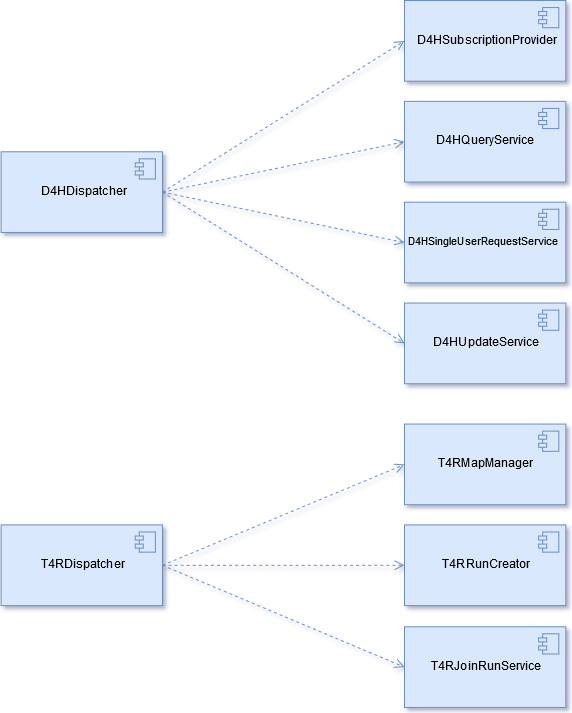
\includegraphics[width=.7\linewidth, keepaspectratio]{./Images/Section5/integration_g4.png}
    \centering
    \caption{Integration group 4}
    \label{fig:intg4}
 \end{figure}

\newpage
\paragraph{High level dispatcher:} the high level dispatcher group is composed by the GenericDispatcher alone, as previously said, and must be integrated with the service dispatchers and the AuthenticationManager. The integration step is hence composed by integrations of the same component with 3 higher (in the hierarchy) components.
\begin{figure}[H]
    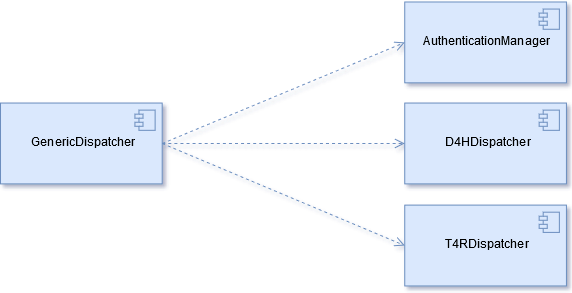
\includegraphics[width=.7\linewidth, keepaspectratio]{./Images/Section5/integration_g5.png}
    \centering
    \caption{Integration group 5}
    \label{fig:intg5}
 \end{figure}

\paragraph{EntryPoint:} the entry point is the last subcomponent to be integrated, and has to be integrated only with the GenericDispatcher, as its task is to analyze incoming packets and forward them to the dispatcher if complete and correct.
\begin{figure}[H]
    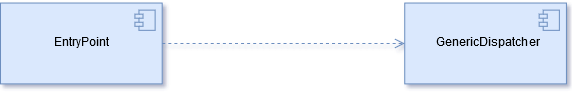
\includegraphics[width=.7\linewidth, keepaspectratio]{./Images/Section5/integration_g6.png}
    \centering
    \caption{Integration group 6}
    \label{fig:intg6}
 \end{figure}

\newpage
\paragraph{TrackMe client applications:} this last group is formed by higher level component, which are the various TrackMe client applications. At this point the server application is fully integrated and the applications require to be integrated with it. This is the last step of integration.
\begin{figure}[H]
    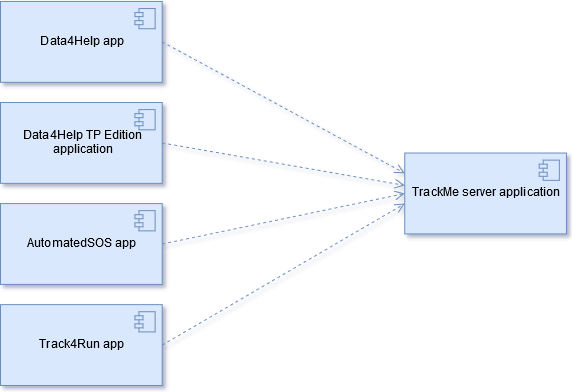
\includegraphics[width=.7\linewidth, keepaspectratio]{./Images/Section5/integration_g7.png}
    \centering
    \caption{Integration group 7}
    \label{fig:intg7}
 \end{figure}

%%%%
{\color{secblue}\subsubsection{Integration test plan}}
The adopted integration test strategy is a bottom-up approach, given the already mentioned structure of the system. For each group of implementation, the single units will be tested through the creation of drivers, which have to test the most possible and most critical cases. In this sense, while building the system, a white-box approach will be used for each single subcomponent. This means that each subcomponent will have a driver to test its functionalities. Such driver will be replaced when integrated to the actual subcomponent. This approach allows to find more easily errors and critical task concerning single components.
\newline Is advised that the integration between subcomponents is done only after a full test is performed successfully on the subcomponent offering the interface. In this way is assumed that the subcomponent on which the new subcomponent relies is fully operative: testing can be hence done on the newer subcomponent with a new driver.
\newline Is also to notice that, having been grouped up the server application subcomponents in the integration plan, the testing on each component in a group can be done indipendently, as subcomponents in the same group never depend one on another.

\paragraph{} When the server application will be completed, a black-box test will be required. This will be done for different reasons:
\begin{itemize}
\item A global test is required to acknowledge the correct integration of the whole system.
\item A black-box approach allows to eventually find different kinds of problems which could not emerge in white-box testing for single units, such as bottlenecks in the system.
\item A stress test is required to test the elasticity of the server application, which has to be flexible and allocate dynamically resources based on the number of the requests received.
\end{itemize}
